\documentclass{standalone}
\begin{document}
\subsection{Pre-processing}

This preliminary step is performed before the training and segmentation process.
It involves the application of a smoothing filter to remove noise which can be a source of false positive in the classification of pixels and a gamma correction filtering to increase the brightness of the images.\\
First of all, for each patient, the MRI scans are read with the original pixel depth, that is 16-bit integers, in order to preserve all the original information.
Then, to have pixel data in the range $ [ 0, \: 1 ] $, images are normalized and rescaled to binary floating point 32-bit, required to work with \textsc{TensorFlow}\cite{Tensorflow} and \textsc{Keras} API\cite{Keras}.
Moreover, if the image size does not match the most common one which is $512 \times 512$ pixels, the image is resized to the latter in order to have the same image size for all the images. 
\\
The images are filtered to remove noise, using the non-local means algorithm from \textsc{Scikit-Image}\cite{scikit-image} library.
The non-local means algorithm replaces the value of a pixel by an average of a selection of other pixels values: 
small patches centered on the other pixels are compared to the patch centered on the pixel of interest, and the average is performed only for pixels that have patches close to the current patch. 
As a result, this algorithm can restore well textures, that would be blurred by other denoising algorithm\cite{scikit-image}.
In Figure \ref{noisydenoised}, you can see the result of the non-local means algorithm on the same MR image of a patient affected by colorectal cancer.
The original image on the \textit{left}, is affected by noise while the filtered one, on the \textit{right}, results in less noise and is smoothed without significant detail loss. 
In fact, one drawback of smoothing filters is the blurring of small details but in this case, they are preserved.
This behavior is reflected in the image histogram. 
As you can see in Figure \ref{histo}, the original image histogram (red) presents great fluctuations of pixel intensity, that highlight the presence of noise. 
Instead, the denoised image histogram (blue) results in a smoothed histogram preserving the original shape.
\\
After denoising, the image brightness is enhanced using a gamma correction.
It consists of a non-linear operation, defined in the simplest cases, by the following power-law expression:
\begin{equation}
    I_{out} = C I_{in}^{\gamma}
\end{equation}
where the output $I_{out}$ is obtained multiplying by a constant $C$ the input value $I_{in}$ raised to the power $\gamma$.
In this case, the gamma correction was achieved by the following expression: 
\begin{equation}
    I_{out} =  (\frac{I_{in} - I_{min}}{I_{max} - I_{min}})^{\gamma}
\end{equation}
where $I_{min}, \: I_{max}$ are respectively the minimum and the maximum image value.
The reason for the gamma correction is, as above mentioned, to increase the brightness of the image, especially for the center of the image which is our region of interest (i.e. the tumor region) and it is often quite dark.
The result of the gamma correction can be seen in Figure \ref{denoisedgamma}.
The increase of brightness is also visible on the gamma-corrected image histogram, shown in Figure \ref{histogamma}.
\\
In summary, the preprocessing steps are:
\begin{itemize}
    \item normalization and rescaling
    \item denoising
    \item gamma correction
\end{itemize}
The comparison of the image before and after the pre-processing can be seen in Figure\ref{noisyfinal}.



\begin{figure}[htp]

    \centering
    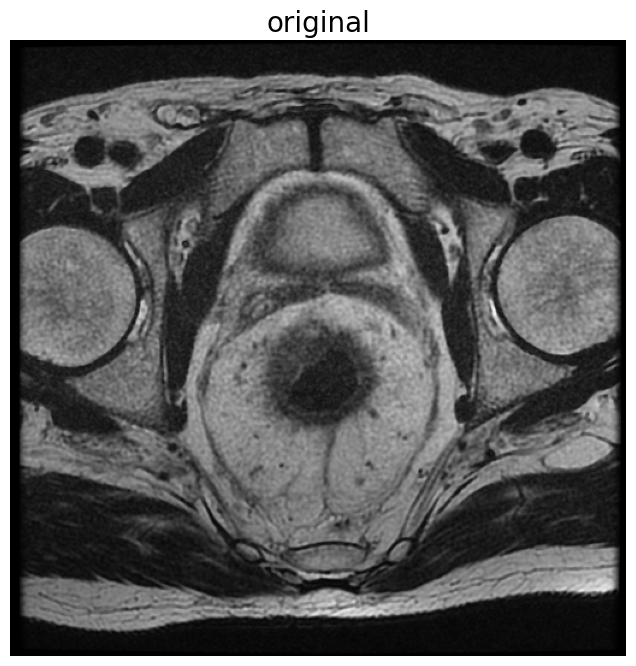
\includegraphics[width=.49\textwidth]{../images/noisy.png}
    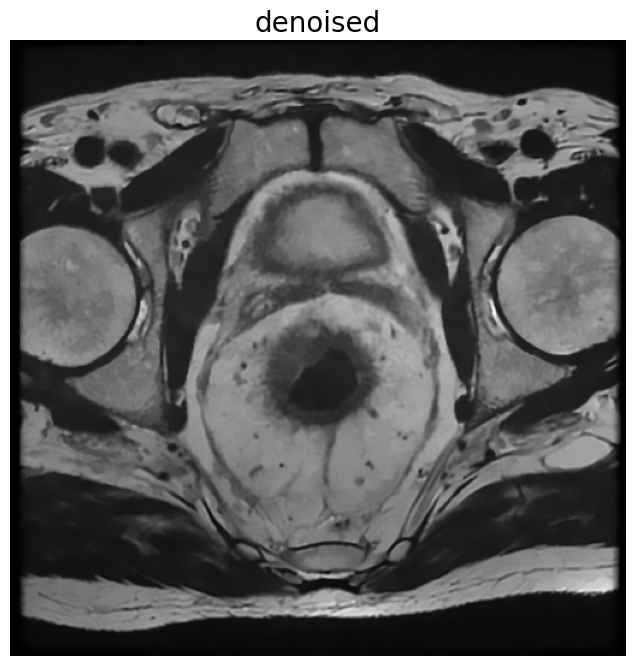
\includegraphics[width=.49\textwidth]{../images/denoised.png}
    
    \caption{ \textit{ Left)} Original MR image of a patient affected by colorectal cancer.\textit{ Right)} The same image after non-local mean algorithm.}
    \label{noisydenoised}
    
    \end{figure}

\begin{figure}[htp]

    \centering
    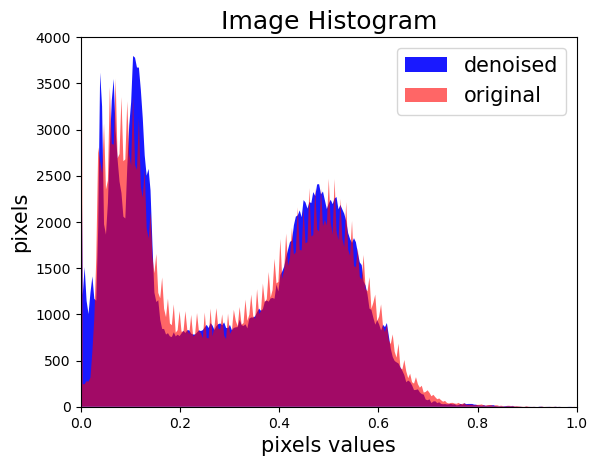
\includegraphics[width=0.73\textwidth]{../images/histogram.png}

    
    \caption{Original vs denoised image histogram. The original image histogram (red) presents great fluctuations of pixel intensity, highlighting the presence of noise. The denoised image one (blue) results in a smoothed histogram preserving the original shape.}
    \label{histo}
    
    \end{figure}

\begin{figure}[htp]

    \centering
    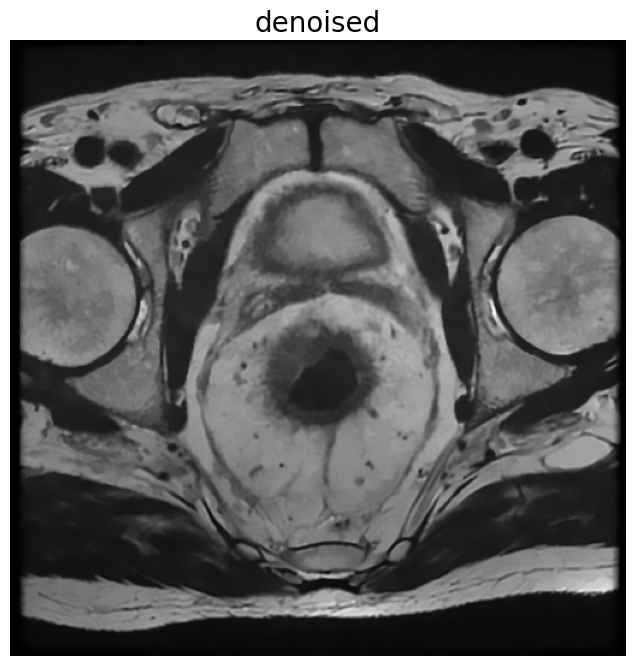
\includegraphics[width=.49\textwidth]{../images/denoised.png}
    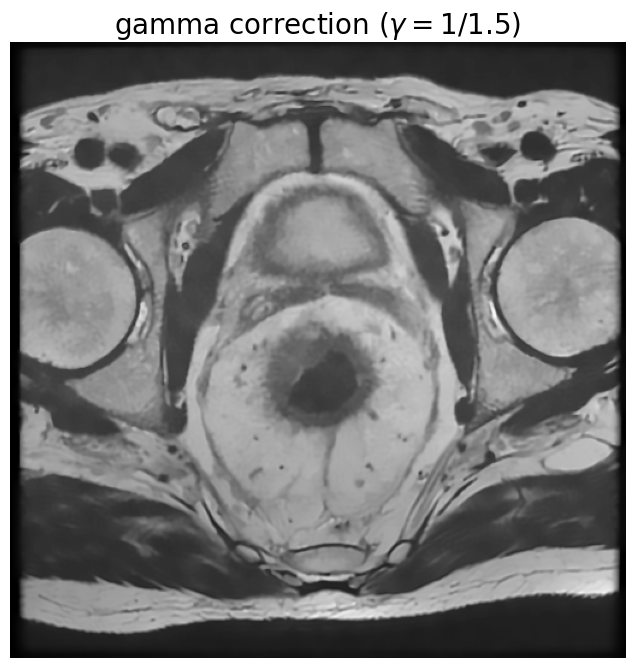
\includegraphics[width=.49\textwidth]{../images/gammacorrection.png}
    
    \caption{ \textit{ Left)} denoised MR image of a patient affected by colorectal cancer.\textit{ Right)} The same image after gamma correction.}
    \label{denoisedgamma}
    
    \end{figure}

\begin{figure}[htp]

    \centering
    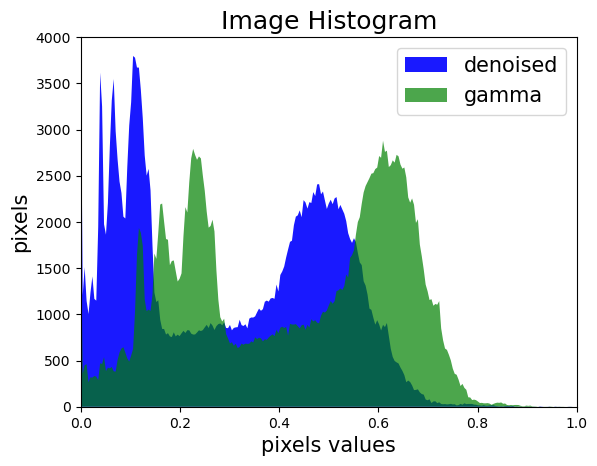
\includegraphics[width=0.73\textwidth]{../images/gammahist.png}

    
    \caption{Denoised vs gamma-corrected image histogram. The gamma-corrected image histogram (green) results in a right-shifted histogram,  thus in increased brightness.}
    \label{histogamma}
    
    \end{figure}

\begin{figure}[htp]

    \centering
    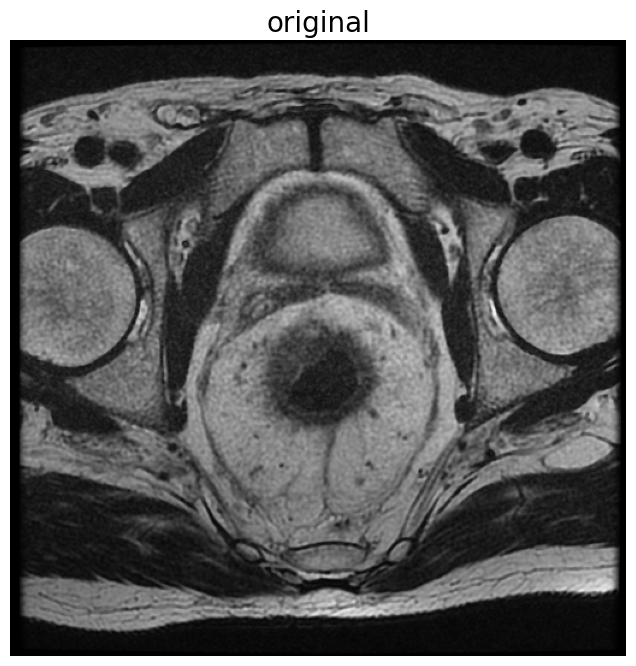
\includegraphics[width=.49\textwidth]{../images/noisy.png}
    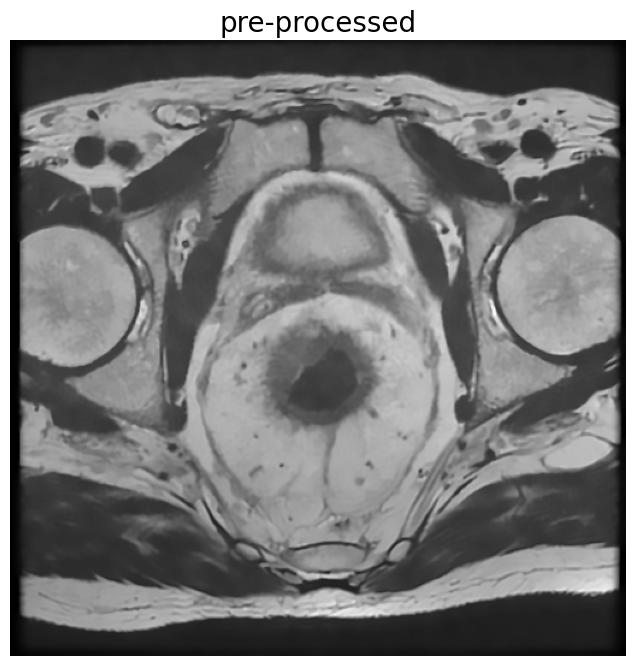
\includegraphics[width=.49\textwidth]{../images/finalimage.png}
    
    \caption{ \textit{ Left)} Original MR image of a patient affected by colorectal cancer.\textit{ Right)} The same image after the pre-processing steps.}
    \label{noisyfinal}
    
    \end{figure}
\end{document}